%!TEX root = ../report.tex

\chapter{ State of the Art }

Given the range of the different methods for implementing a spatio-temporal
world model, the methods have been divided into groups.  Most spatio-temporal
world models are implemented on top of preexisting world modeling techniques
and thus the majority of implementations are tied to a specific spatial
representation. There are, however, exceptions to this with some models being
built from the ground up effectively intertwining the spatial and temporal
components. On the opposite end of this spectrum, there exists currently at
least one method that can be used in combination with a multitude of different
world models.


\section{ Map Dependent Models }

\subsection{ Occupancy Grids }

Occupancy grids were introduced in 1985 by Moravec and Elfes. \cite{Elfes1985}
In simple two dimensional terms, they can be thought of as a grid placed
over an environment. Each cell then represents the probability or belief that
that that cell is either occupied or free. Free in the simplest case meaning
that a robot would be able to traverse through the cell. This concept can of
course be extended into the third dimension for a more complex world model. \\

\subsubsection{ Temporal Occupancy Grids }
One of the earliest and most straight forward attempts to introduce a temporal
component to a world model were by extending existing world models, occupancy
grids in particular. This can be seen in Temporal Occupancy Grids: a Method for
Classifying the Spatio-Temporal Properties of the Environment.
\cite{Arbuckle2002} In this paper Arbuckle et al introduce the concept of
temporal occupancy grids (TOGs). The authors noted that the key to these TOGs
were that they "can differentiate between different patterns of occupancy, even
when the absolute probability of occupancy is the same." That is to say, one
could imagine a parking lot where it would be possible with TOGs to distinguish
between cells that are parking spaces, cells that are pathways, and cells that
are not for driving at all, such as a median. These TOGs additionally made it
possible to detect where a door or elevator may be. \\

Temporal Occupancy Grids were accomplished by generated multiple occupancy
grids in the same fashion as was traditionally done but each occupancy grid
would represent, and be generated using samples from, multiple different time
scales. With multiple occupancy grids spanning multiple time scales, the
probability of a cell being occupied could be computed by a simple summation.

\subsubsection{ Hidden Markov Models }

Hidden Markov Models (HHMs), are a type of Markov Chain that can be considered
"a doubly embedded stochastic process with an underlying stochastic process
that is not observable (it is hidden), but can only be observed through
another set of stochastic processes that produce the sequence of observations."
\cite{Rabiner1989}. In more general terms, an HMM can be though of as having N
number of states S, that are hidden, or otherwise not directly observable.
Each state can have M observations made about properties of these states which
may reflect indirectly, to varying degrees of certainty, the actual state.
Furthermore, each one of these states has a given probability distribution of
transitioning from one state to another. It is from this information that a
Markov Model or Markov Chain can be constructed. \\

TODO: Add image? \\

In the specific case of occupancy grids, each cell can be thought of having two
states, free, and occupied. It is not feasible to be able to directly observe
every given cell at all times, and specifically at the time of path planning
and thus there states can be thought of as hidden. However, through past
observation and data collection, there is data know about a cell throughout
time. Thus this temporal data can be thought of as the observational data and
be used to make predictions about state transitions. \\

Early combinations of HMMs with occupancy grids differed from previous dynamic
world modeling approaches as this approach "does not depend on dynamic object
detection and high-level object models; it considers only the occupancy of the
space at a lower level of abstraction"\cite{Meyer-Delius2012}. By relying on
and collecting lower, more easily observable data, larger amounts of data could
be collected and processed over greater periods of time. Since each cell was
dependent only on previous observations of that cell throughout time, the
increase in data quantity and the discrete nature of the predictions lent
themselves would improve state predictions. \\

Meyer-Delius \cite{Meyer-Delius2012} also introduced the concept of online
learning to this approach. Traditionally, offline learning had been used where
a robots navigational system would hold copy of a world model produced a some
time before operation. It has possible that from the time the map was generated
to the time at which the robot was operating that objects in the robots
environment may have changed. With the introduction of online learning, the
robot would be able to observe these changes and factor them in to its
navigational system. This was the first addition to attempt to avoid the static
nature of the transition states of the HMM. \\

Further improvement to occupancy grids with HMMs came with the concept of
modeling trajectories of objects in the environment\cite{Wang2015}. This is an
important improvement because the dynamic motion of objects in an environment,
such as humans walking a hallway, could now be better modeled. This process
was dubbed Input-Output HMM (IOHMM) due nature of how cells of the grid would
communicate with one another. Each cell would not only look through it's own
historical data but also be able to communicate with its neighbors. In effect,
this could allow a cell in hallway to be able to predict occupancy based off of
a nearby cell that is currently occupied.

\subsection{ Spatio-Temporal Hilbert Maps }

\begin{figure}[!htb]
  \centering
  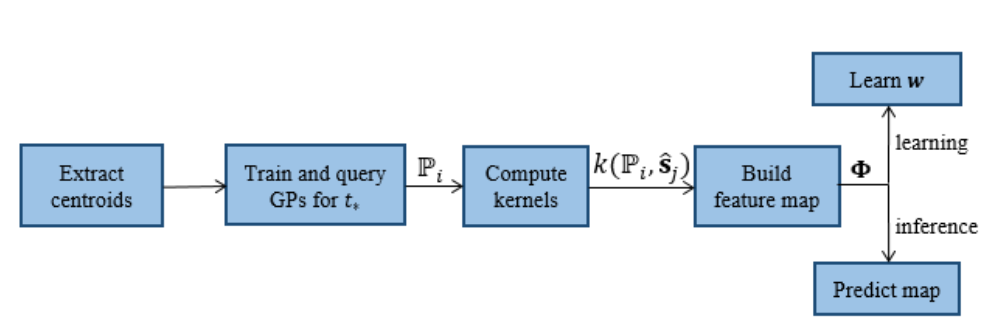
\includegraphics[width=\linewidth]{images/STHM_diag.png}
  \caption{Spatio-temporal Hilbert map training process (GP - Gaussian Process)}
  \cite{Senanayake2016}
  \label{figure:STHM}
\end{figure}

In contrast to the discrete nature of occupancy grids, Hilbert maps provide a
continuous representation of an environment which allows for arbitrary world
model resolution. They rely on "fast kernel approximations that project the
data in a Hilbert space where a logistic regression classifier is learnt"
A stochastic gradient optimization can then applied. This approach is similar to
that of a Gaussian processes occupancy map but with a much lower computational
cost computational cost computational cost computational cost. Having been
introduced as recently as 2016, Hilbert maps, and the addition of a temporal
component, are still a fairly new field of research but already some of the
authors from the original paper have already begun to introduce a temporal
component to this new form of world model. \cite{Ramos2016, Senanayake2016} \\

In static Hilbert maps, the kernel can be thought of as the location of an
obstacle or object. When introducing the temporal dimension, the centroid of a
moving object is extracted from raw data over time. This data can the be used
and trained on to create a model that can predict the direction and speed of an
object at a given location at a given time. It is particularly well suited to
short-term predictions such as car traffic on a road or at an intersection.
\cite{Senanayake2016} \cite{Senanayake2017}

\section{ Map Independent Models }

\subsection{ FreMen }

Frequency Map Enhancement, or FreMEn as it became known, is a technique for
spatio-temporal world modeling that can be used independent of mapping or
world modeling technique. It was introduced by Tomáš Krajník, Jaime Pulido
Fentanes, Grzegorz Cielniak, Christian Dondrup, an Tom Duckett in 2014. It's
original goals focused on improving mapping for long-term scenarios.
Additionally, it was notice that a large number of previous approaches had
focused on mapping multiple static environments over time which worked well
for environments that changed slowly, but were not necessarily well fit for
highly dynamic environments. FreMEn was designed to counter these issues.
\cite{Fentanes2014} Although initially used with octomaps, three dimensional
occupancy grids, it was later decoupled from this mapping technique allowing
it to be an extremely diverse and flexible technique. \\

In it's original and most basic form, FreMEn assumes that an environment can be
broken down into multiple independent components. It is then further assumed
that these independent components will take one of two binary states. Examples
of this include a door being open or shut, a room being occupied, or a cell in
an occupancy grid being free or occupied. Each one of these states can not
always be directly observed, and the tools e.g. sensors available to the robot
my have noise and cannot be taken as one hundred percent ground truth. Thus,
each one of these components has a certain probability assigned to it. This
probability defines the likelihood of it being in a given state, e.g. a door
open or closed.  Finally, since these states can be observed multiple times
over a given period of time, their probabilities can then be defined as
functions dependent on time. \\

At the heart of FreMEn lies a well known mathematical tool commonly used for
signal processing, the Fourier Transform. Since FreMEn focuses on long term
observations of dynamic, often human, environments, it is assumed that harmonic
patterns will develop over time. The Fourier Transform can then be applied to
these long term observations to convert them into the spectral domain for
storage. Furthermore, because the Fourier Transform is easily reversible,
with the inverse Fourier Transform, one can easily convert between the stored
observations in the spectral domain back to the time domain. This allows for
predictions at any given time t. Not only is this extremely useful for future
predictions, but this method can also be used to analyze the accuracy of the
model by comparing previously observed data from the past to the models
predictions. Using this historical accuracy one can then tune the order of the
spectral model to obtain more accurate historical predictions with hopes of
also having more accurate future predictions. More information on this process
can be found in the original paper\cite{Fentanes2014} and the follow up FreMEn
paper \cite{Krajnik2015}. \\

\subsubsection{ Improvements and Additions }

As ground breaking and as flexible as FreMEn is, due to the many assumptions
made, it is not without its flaws. One major assumption made is that areas of
observation can be observed not only frequently but periodically in the most
strict sense. That is to say, it is not only important that a location be
visited and observed, but that the observations follow a pattern of equally
spaced and timed observations. This is due to the Fast Fourier Transform (FFT)
technique that is used in the original papers. Thus, latter authors devised and
implemented other methods of storing data and making predictions. This often
involved phase shifting or modifying the amplitude of the observation as well
as using a modified equation derived from the Fourier Transform instead of the
standard FFT. More information can be found in the paper \cite{Santos2016}. \\

Another major limitation of FreMEn is its assumption that all observable
behavior can be modeled with binary states. An  attempt to solve this issue
was to replace the Bernoulli distribution of FreMen with the specific hope of
being able to better represent human patterns present in environment such as
an office building or hospital. Specifically, they "extend the technique
(FreMEn) by employing both Poisson processes as the counting model to replace
the binary states of FreMEn and a new way of selecting the most prominent
frequency components of the Fourier spectrum."\cite{Jovan2016} This approach,
however, does not come without its own set of assumptions. Since human
activity is assumed, the authors also assume behavior would be best grouped by
the work week. For example, data sampled for a two months would be broken into
8 week sections. This works extremely well for patterns that are persistent on
a weekly basis but perhaps not as well for seasonal changes for example. At
the very least, one must apply some critical thinking to how data should be
group depending on the desired application.


\begin{figure}[!htb]
  \centering
  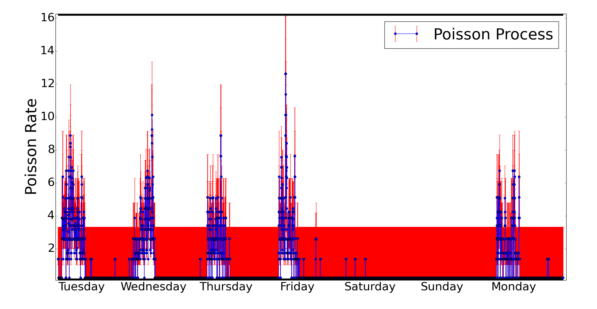
\includegraphics[width=\linewidth]{images/poisson-spectral-process.png}
  \caption{Lambda time series of a corridor using Poisson Process}
  \cite{Jovan2016}
  \label{figure:PSP}
\end{figure}

TODO: perhaps a section about the different FreMEn applications available e.g.
FreMEn grids, FroctoMaps etc

\section{ Existing Methods for Evaluation or Comparison }

\subsection{ Current Methods }
\subsection { Example 1 }
\subsection { Example 2 }

\subsection{ Limitations and Areas of Oversight }
